\documentclass{article}
\usepackage[margin=1in]{geometry}
\usepackage{pgf}
\usepackage{tikz}
\usetikzlibrary{arrows,automata}
\usepackage[latin1]{inputenc}
\usepackage{listings}
\lstdefinestyle{customc}{
  belowcaptionskip=1\baselineskip,
  breaklines=true,
  frame=L,
  xleftmargin=\parindent,
  language=C,
  showstringspaces=false,
  basicstyle=\footnotesize\ttfamily,
  keywordstyle=\bfseries\color{green!40!black},
  commentstyle=\itshape\color{purple!40!black},
  identifierstyle=\color{blue},
  stringstyle=\color{orange},
}
\lstset{escapechar=@,style=customc}

\newcommand\D{4}

\begin{document}

\lstinputlisting[caption=page\_check\_references, style=customc]{src/page_check_references.c}
\newpage

\lstinputlisting[caption=shrink\_page\_list, style=customc]{src/simple_shrink_page_list.c}
\newpage

\begin{figure}
\center
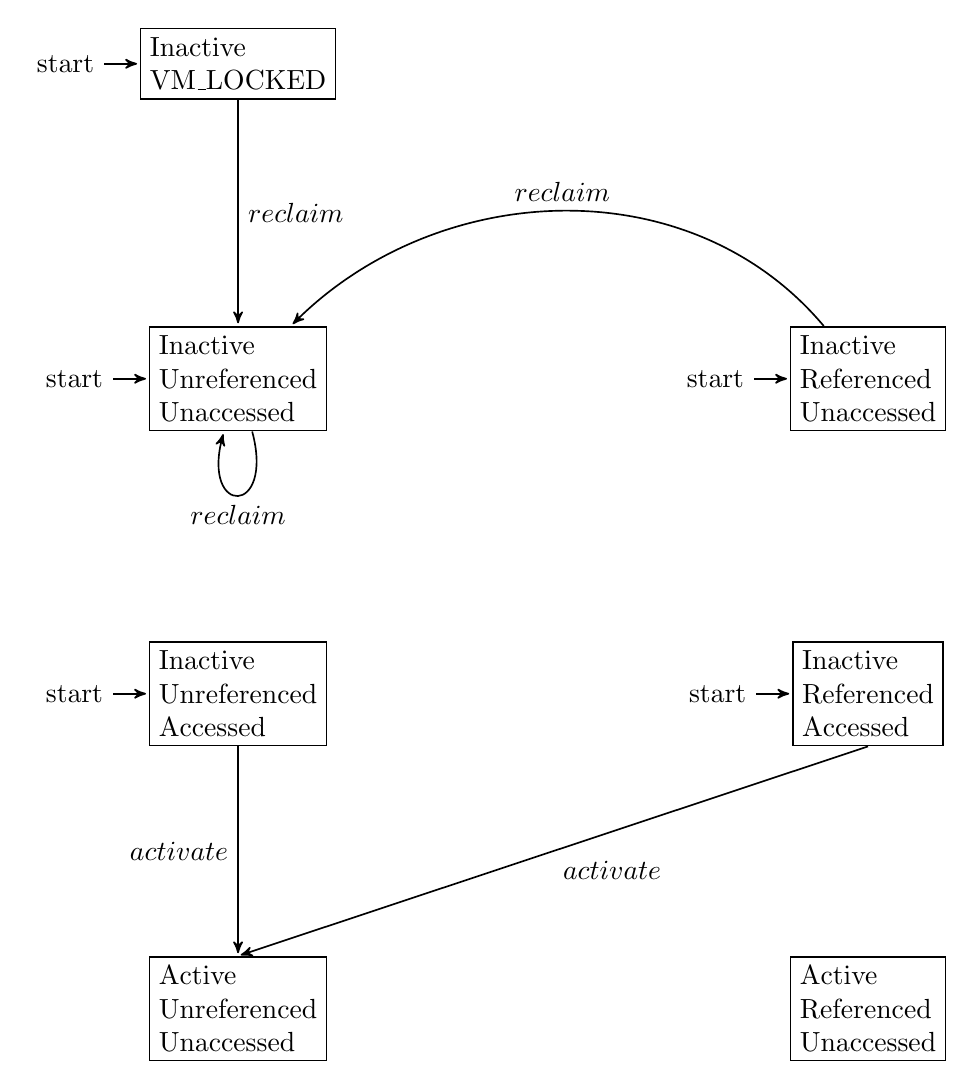
\begin{tikzpicture}[->,>=stealth',shorten >=1pt,auto,node distance=\D{}cm,
                    semithick]

  \tikzstyle{every state}=[rectangle,draw,align=left]

  \node[initial,state] (IUU) at (0,0)        {Inactive \\ Unreferenced \\ Unaccessed};
  \node[initial,state] (IRU) at (2*\D,0)     {Inactive \\ Referenced   \\ Unaccessed};
  \node[initial,state] (LCK) at (0,\D)       {Inactive \\ VM\_LOCKED};
  \node[initial,state] (IUA) at (0,-\D)      {Inactive \\ Unreferenced \\ Accessed};
  \node[initial,state] (IRA) at (2*\D,-\D)   {Inactive \\ Referenced   \\ Accessed};
  %\node[initial,state] (IAA) at (\D,-\D)     {Inactive \\ Unreferenced \\ Accessed $>$ 1};
  \node[state]         (AUU) at (0,-2*\D)    {Active   \\ Unreferenced \\ Unaccessed};
  \node[state]         (ARU) at (2*\D,-2*\D) {Active   \\ Referenced   \\ Unaccessed};

  \path
  (LCK) edge [out=270,in=90,looseness=0]      node {$reclaim$} (IUU)
  (IUU) edge [loop below]                     node {$reclaim$} (IUU)
  (IRU) edge [out=130,in=45,looseness=1,swap] node {$reclaim$} (IUU)

  (IUA) edge [out=270,in=90,looseness=0,swap] node {$activate$} (AUU)
  (IRA) edge [out=270,in=90,looseness=0]      node {$activate$} (AUU)
  ;
\end{tikzpicture}
\caption{Anon LRU Automata}
\end{figure}

\begin{figure}
\center
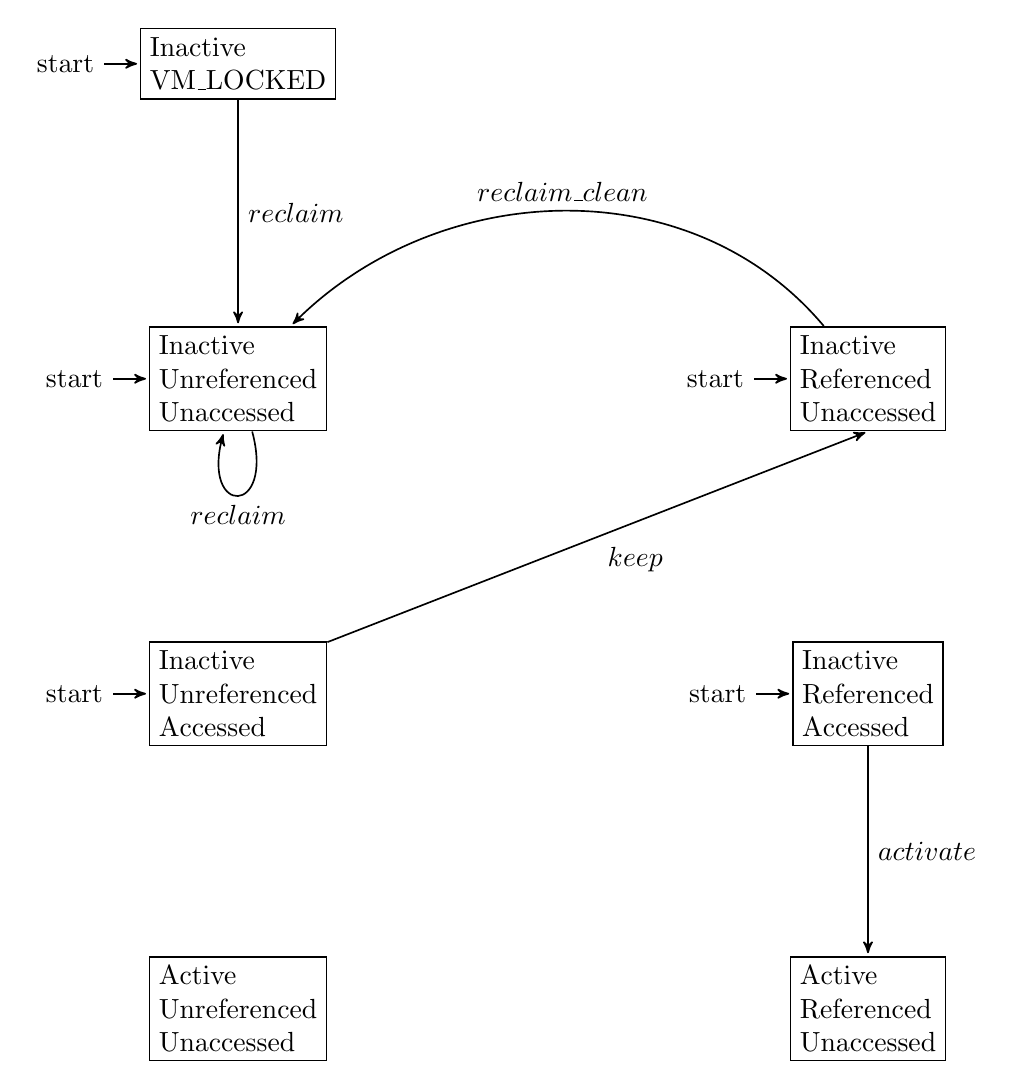
\begin{tikzpicture}[->,>=stealth',shorten >=1pt,auto,node distance=\D{}cm,
                    semithick]

  \tikzstyle{every state}=[rectangle,draw,align=left]

  \node[initial,state] (IUU) at (0,0)        {Inactive \\ Unreferenced \\ Unaccessed};
  \node[initial,state] (IRU) at (2*\D,0)     {Inactive \\ Referenced   \\ Unaccessed};
  \node[initial,state] (LCK) at (0,\D)       {Inactive \\ VM\_LOCKED};
  \node[initial,state] (IUA) at (0,-\D)      {Inactive \\ Unreferenced \\ Accessed};
  \node[initial,state] (IRA) at (2*\D,-\D)   {Inactive \\ Referenced   \\ Accessed};
  %\node[initial,state] (IAA) at (\D,-\D)     {Inactive \\ Unreferenced \\ Accessed $>$ 1};
  \node[state]         (AUU) at (0,-2*\D)    {Active   \\ Unreferenced \\ Unaccessed};
  \node[state]         (ARU) at (2*\D,-2*\D) {Active   \\ Referenced   \\ Unaccessed};

  \path
  (LCK) edge [out=270,in=90,looseness=0]      node {$reclaim$} (IUU)
  (IUU) edge [loop below]                     node {$reclaim$} (IUU)
  (IRU) edge [out=130,in=45,looseness=1,swap] node {$reclaim\_clean$} (IUU)

  (IUA) edge [in=270,out=30,looseness=0,swap] node {$keep$} (IRU)
  (IRA) edge [out=270,in=90,looseness=0]      node {$activate$} (ARU)
  ;
\end{tikzpicture}
\caption{File LRU Automata}
\end{figure}

\begin{figure}
\center
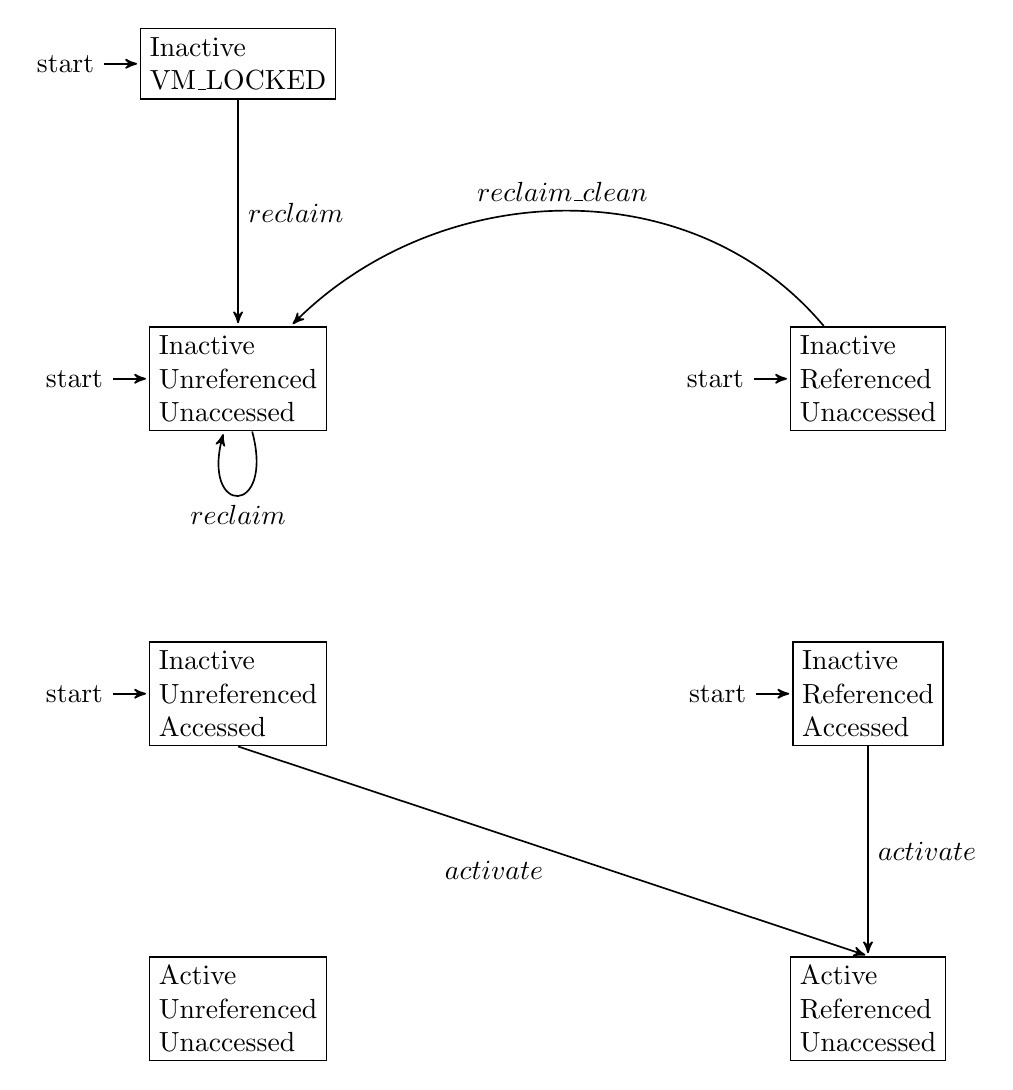
\begin{tikzpicture}[->,>=stealth',shorten >=1pt,auto,node distance=\D{}cm,
                    semithick]

  \tikzstyle{every state}=[rectangle,draw,align=left]

  \node[initial,state] (IUU) at (0,0)        {Inactive \\ Unreferenced \\ Unaccessed};
  \node[initial,state] (IRU) at (2*\D,0)     {Inactive \\ Referenced   \\ Unaccessed};
  \node[initial,state] (LCK) at (0,\D)       {Inactive \\ VM\_LOCKED};
  \node[initial,state] (IUA) at (0,-\D)      {Inactive \\ Unreferenced \\ Accessed};
  \node[initial,state] (IRA) at (2*\D,-\D)   {Inactive \\ Referenced   \\ Accessed};
  %\node[initial,state] (IAA) at (\D,-\D)     {Inactive \\ Unreferenced \\ Accessed $>$ 1};
  \node[state]         (AUU) at (0,-2*\D)    {Active   \\ Unreferenced \\ Unaccessed};
  \node[state]         (ARU) at (2*\D,-2*\D) {Active   \\ Referenced   \\ Unaccessed};

  \path
  (LCK) edge [out=270,in=90,looseness=0]      node {$reclaim$} (IUU)
  (IUU) edge [loop below]                     node {$reclaim$} (IUU)
  (IRU) edge [out=130,in=45,looseness=1,swap] node {$reclaim\_clean$} (IUU)

  (IRA) edge [out=270,in=90,looseness=0]      node {$activate$} (ARU)

  (IUA) edge [in=90,out=270,looseness=0,swap] node {$activate$} (ARU)
  ;
\end{tikzpicture}
\caption{VM\_EXEC File LRU Automata}
\end{figure}

\begin{figure}
\center
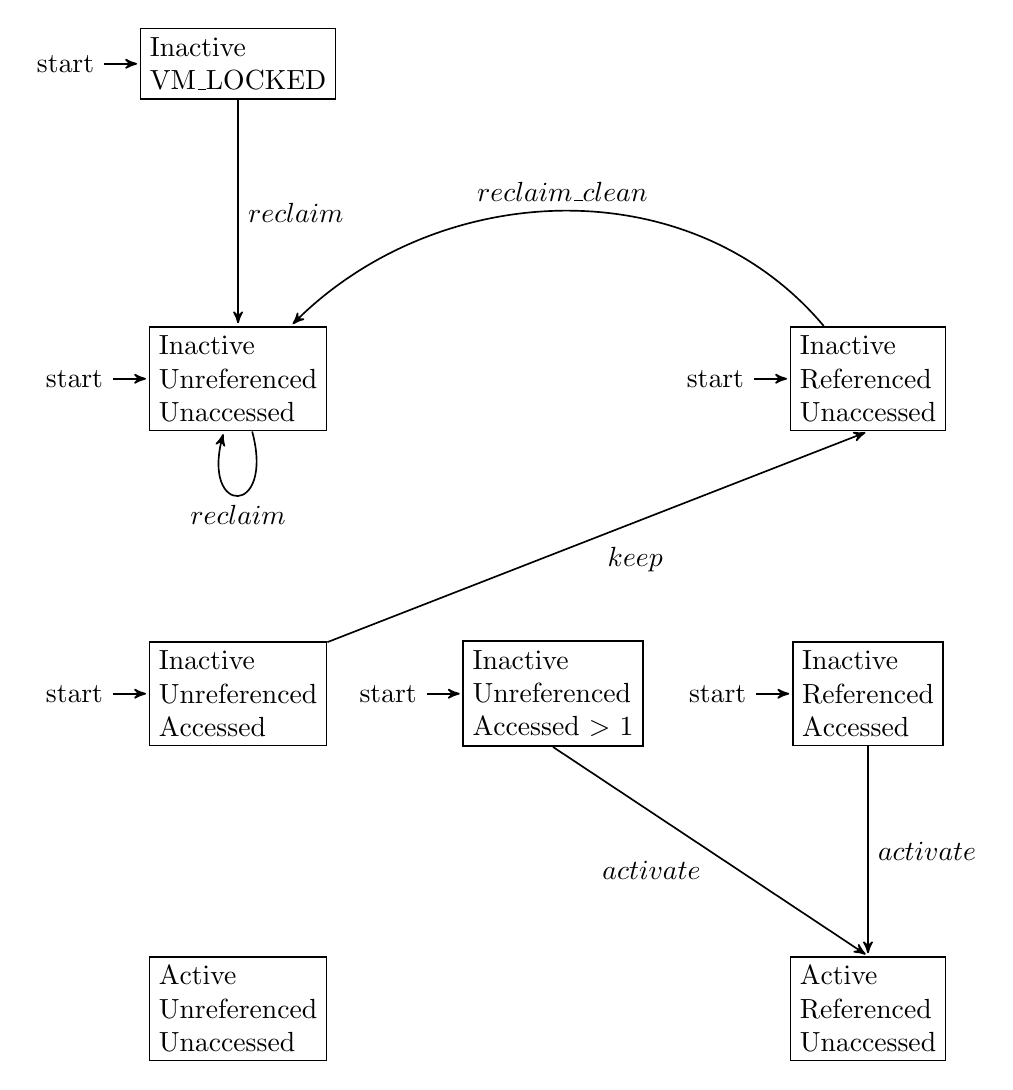
\begin{tikzpicture}[->,>=stealth',shorten >=1pt,auto,node distance=\D{}cm,
                    semithick]

  \tikzstyle{every state}=[rectangle,draw,align=left]

  \node[initial,state] (IUU) at (0,0)        {Inactive \\ Unreferenced \\ Unaccessed};
  \node[initial,state] (IRU) at (2*\D,0)     {Inactive \\ Referenced   \\ Unaccessed};
  \node[initial,state] (LCK) at (0,\D)       {Inactive \\ VM\_LOCKED};
  \node[initial,state] (IUA) at (0,-\D)      {Inactive \\ Unreferenced \\ Accessed};
  \node[initial,state] (IRA) at (2*\D,-\D)   {Inactive \\ Referenced   \\ Accessed};
  \node[initial,state] (IAA) at (\D,-\D)     {Inactive \\ Unreferenced \\ Accessed $>$ 1};
  \node[state]         (AUU) at (0,-2*\D)    {Active   \\ Unreferenced \\ Unaccessed};
  \node[state]         (ARU) at (2*\D,-2*\D) {Active   \\ Referenced   \\ Unaccessed};

  \path
  (LCK) edge [out=270,in=90,looseness=0]      node {$reclaim$} (IUU)
  (IUU) edge [loop below]                     node {$reclaim$} (IUU)
  (IRU) edge [out=130,in=45,looseness=1,swap] node {$reclaim\_clean$} (IUU)

  (IUA) edge [in=270,out=30,looseness=0,swap] node {$keep$} (IRU)
  (IRA) edge [out=270,in=90,looseness=0]      node {$activate$} (ARU)

  (IAA) edge [in=90,out=270,looseness=0,swap] node {$activate$} (ARU)
  ;
\end{tikzpicture}
\caption{Shmem File LRU Automata}
\end{figure}

\end{document}
